\documentclass[tikz,border=6pt]{standalone}
\usepackage{amsmath}
\usepackage{bm}
\usetikzlibrary{arrows.meta,decorations.markings,calc}

\begin{document}
	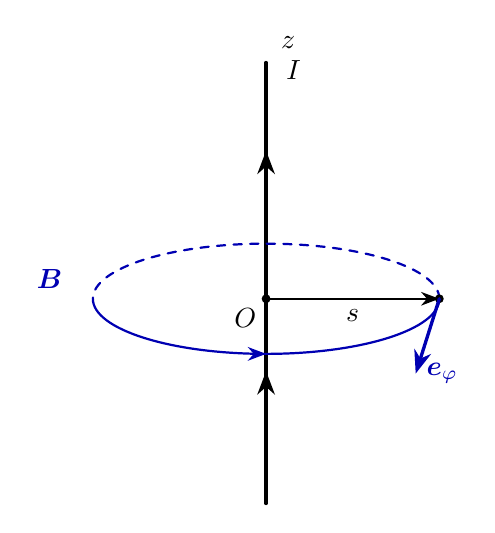
\begin{tikzpicture}[>=Stealth,line cap=round,scale=1.0]
		
		% ===== 透视参数：z 轴竖直，xy 平面用斜投影画成椭圆 =====
		% 椭圆：水平半轴 a，竖直半轴 b（透视压扁）
		\def\a{2.2}\def\b{0.7}
		
		% ---- 载流细导线（z 轴）----
		\draw[very thick,
		postaction={decorate},
		decoration={markings,
			mark=at position 0.30 with {\arrow{Stealth}},
			mark=at position 0.80 with {\arrow{Stealth}}}]
		(0,-2.6) -- (0,3.0);
		\node at (0.35,2.9) {$I$};
		\node at (0.28,3.25) {$z$};
		
		% ---- 原点 O ----
		\fill (0,0) circle (1.6pt);
		\node[below left] at (0,0) {$O$};
		
		% ---- 磁感线（环绕导线的椭圆，e_phi 方向）----
		% 后半段（被导线挡住的部分）虚线
		\draw[blue!70!black,thick,dashed]
		(\a,0) arc[start angle=0,end angle=180,x radius=\a,y radius=\b];
		% 前半段实线 + 箭头表示 e_phi 环绕方向
		\draw[blue!70!black,thick,
		postaction={decorate},
		decoration={markings,
			mark=at position 0.5 with {\arrow{Stealth}}}]
		(-\a,0) arc[start angle=180,end angle=360,x radius=\a,y radius=\b];
		
		% ---- 场点 P，在 +x 方向距离 s 处（椭圆最右点）----
		\coordinate (P) at (\a,0);
		\fill (P) circle (1.6pt);
		
		% ---- 距离 s（从轴到场点）----
		\draw[->,thick] (0,0) -- (P) node[pos=0.5,below] {$s$};
		
		% ---- e_phi 单位矢量（在 P 处沿环切向，指向纸面前方下侧）----
		\draw[->,very thick,blue!70!black]
		(P) -- ++(-0.3,-0.95)
		node[right] {$\bm{e}_{\varphi}$};
		
		% ---- B 的标注 ----
		\node[blue!70!black] at (-\a-0.55,0.25) {$\bm{B}$};
		
	\end{tikzpicture}
\end{document}